%%%%%%%%%%%%%%%%%%%%%%%%%%%%%%%%%%%%%%%%%%%%%%%%%%%%%%%%%%%%%%%%%%%%%%
%     File: ExtendedAbstract_imple.tex                               %
%     Tex Master: ExtendedAbstract.tex                               %
%                                                                    %
%     Author: Andre Calado Marta                                     %
%     Last modified : 27 Dez 2011                                    %
%%%%%%%%%%%%%%%%%%%%%%%%%%%%%%%%%%%%%%%%%%%%%%%%%%%%%%%%%%%%%%%%%%%%%%
% A Calculation section represents a practical development
% from a theoretical basis.
%%%%%%%%%%%%%%%%%%%%%%%%%%%%%%%%%%%%%%%%%%%%%%%%%%%%%%%%%%%%%%%%%%%%%%

\section{IOb-SoC-Linux Hardware Components}
\label{sec:hardware_developed}

The author had to develop four hardware modules to build a SoC capable of executing a Linux OS. Those hardware modules allowed the integration of a new CPU, a new UART and the hardware needed to support interrupts in the \textit{IOb-SoC}. Besides integrating new hardware in the \textit{IOb-SoC}, minor changes to the \textit{IOb-SoC} core were made. The newly used CPU core was generated based on the \textit{SpinalHDL}~\cite{papon2017spinalhdl} \textit{VexRiscv}~\cite{vexriscv} platform. The \textit{VexRiscv} platform enabled the development of a \textit{VexRiscv} CPU core that meets the requirements of an OS. The \textit{VexRiscv} CPU still needed a CPU wrapper to integrate with the \textit{IOb-SoC} interface. The Linux OS also requires a compatible UART to communicate with the user. Linux has drivers that support an existing \textit{UART16550}. A hardware wrapper allows the integration of the \textit{UART16550} on \textit{IOb-SoC-Linux}. Additionally, the SoC has to support timer and software interrupts to run an OS. The CLINT hardware module developed generates timer and software-related interrupts for a \textit{RISC-V} system. Another hardware component which manages interrupts in a \textit{RISC-V} system is the PLIC. A developed hardware component creates an interface with the \textit{IOb-SoC} and instantiates an existing PLIC core and register modules enabling external interrupts on \textit{IOb-SoC-Linux}. 

Figure~\ref{fig:bd_linux} shows a sketch of the SoC developed.

\begin{figure}[!h]
    \centering
    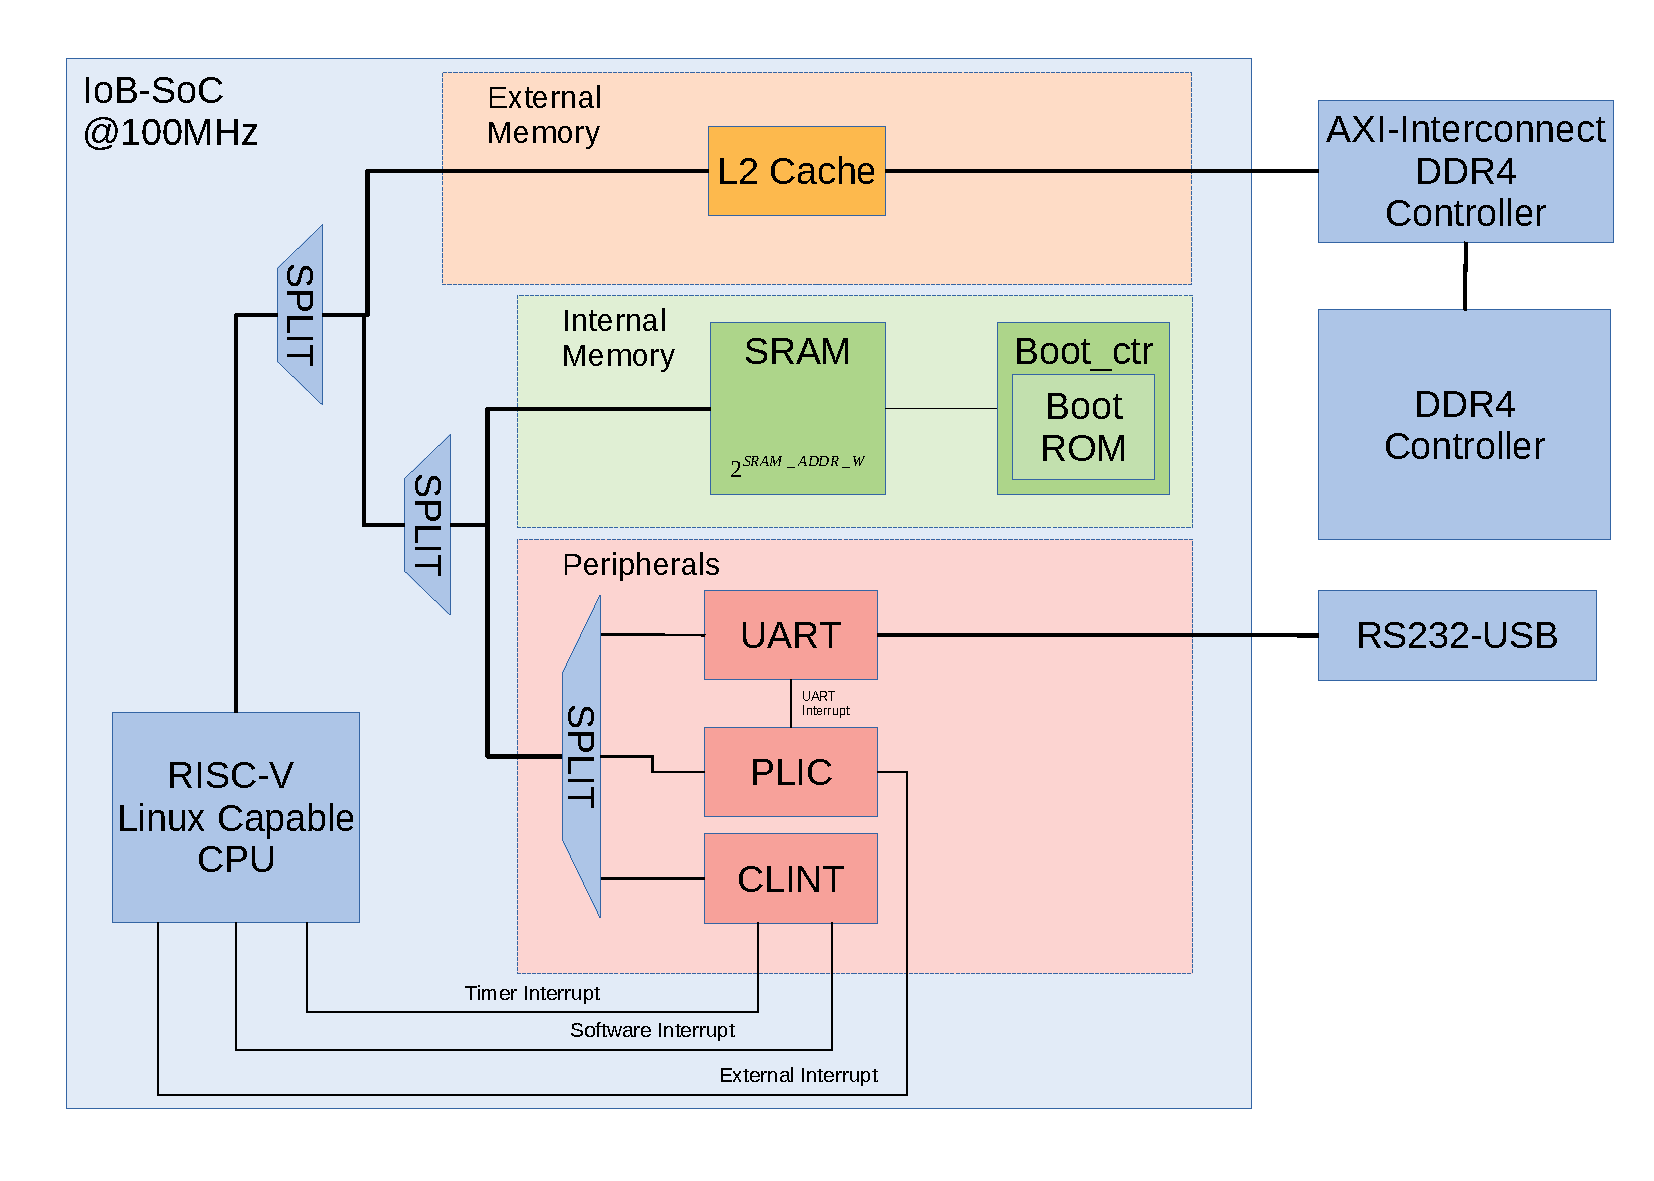
\includegraphics[width=\linewidth]{../images/bd_linux.pdf}
    \caption{Developed SoC sketch.}
    \label{fig:bd_linux}
\end{figure}

\section{Software Components}
\label{sec:software_developed}

During this thesis, the author also developed many software components. Those software components were essential to run a Linux OS in \textit{IOb-SoC} or enhance the \textit{IOb-SoC} platform. First, the new \textit{Console} program written in \textit{Python} allows the \textit{IOb-SoC} platform to communicate through serial with the board. Previously, the \textit{Console} program was written in \textit{C} and had fewer features than the new \textit{Console}. The new \textit{Console} can work with the simulator testbench and communicate with a Linux OS running in \textit{IOb-SoC-Linux}. Secondly, based on the previous \textit{IOb-SoC} verification software, a new hardware simulation testbench can test the SoC and communicate with the \textit{Console} program. Moreover, the \textit{Verilator}~\cite{snyder2010verilator} simulation software allowed the creation of a \textit{Verilator} \textit{C++} testbench to test the SoC faster. Thirdly, a hardware simulation testbench created for the CLINT verifies its behaviour, and a bare-metal interrupt routine firmware developed shows how to use interrupts in \textit{IOb-SoC-Linux}. Finally, the author adapted, built and deployed the software needed to execute a Linux OS in the SoC. The adapted \textit{IOb-SoC} bootloader firmware allows loading the software to the \textit{IOb-SoC-VexRiscv} memory. A device tree file describes the hardware components of the SoC to the Linux kernel. The compiled Linux kernel version must be compatible with the \textit{VexRiscv} CPU, and the root file system developed must be adequate for a minimal Linux OS. While developing the hardware and software components, Makefile scripts helped integrate the components in \textit{IOb-SoC} and automatise the building and deployment process.

Figure \ref{fig:console_flow} presents the \textit{Console} program flowchart.

\begin{figure}[!ht]
    \centering
    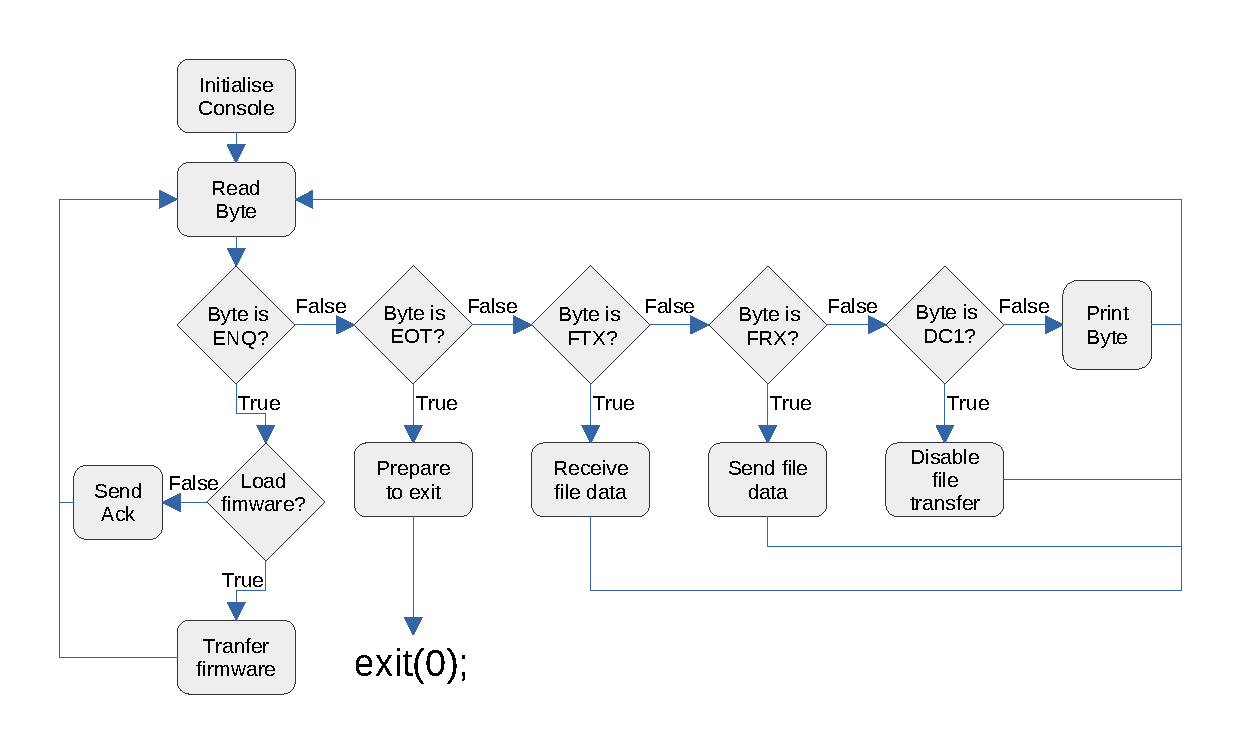
\includegraphics[width=\linewidth]{../images/console_flow.pdf}
    \caption{\textit{Console} program flowchart.}
    \label{fig:console_flow}
\end{figure}

The new verification software interacts with the \textit{Console} through files. Figure~\ref{fig:uut_top_hw} represents a sketch of the verification software and its interaction with the \textit{Console}.

\begin{figure}[!ht]
    \centering
    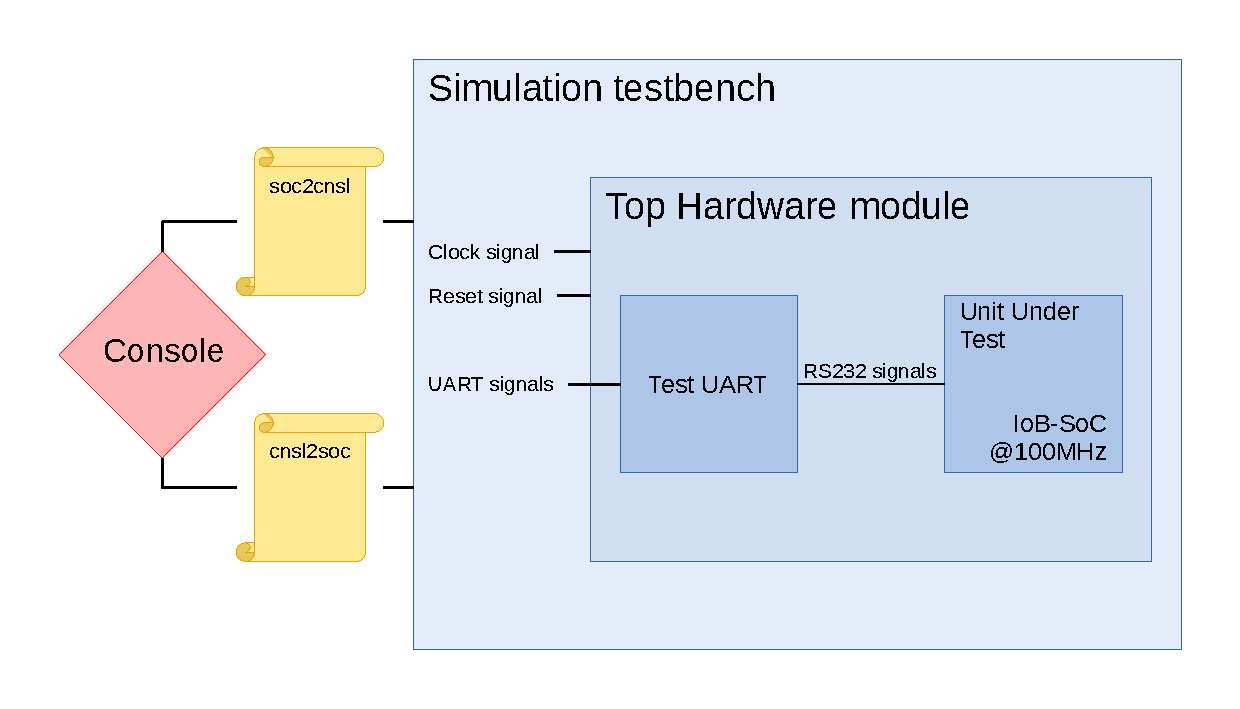
\includegraphics[width=\linewidth]{../images/uut_top_hw.pdf}
    \caption{Simulated hardware interfaces.}
    \label{fig:uut_top_hw}
\end{figure}